\section{Maximum Matchings}
\label{sec:max_matchings}

\newcommand{\maxmatch}{\hyperref[prob:max_matching]{\color{black}\textsf{Maximum Matching}}}
\newcommand{\symdiff}{\ensuremath{\bigtriangleup}}

%\subsection{Introduction and Notation}

\begin{definition}[Matching]
    Given a graph $G = (V, E)$, a matching $M \sse E$ is a set of edges such that no two edges in $M$ share 
    a common vertex. 
    \label{def:matching}
    \begin{definition}[Covered/Exposed]
        A node is $M$-covered if some edge in $M$ is incident to it. Else it is $M$-exposed. 
    \end{definition}
\end{definition}

Note that a matching $M$ covers exactly $2\abs{M}$ nodes, leaving $\abs{V} - 2\abs{M}$ nodes exposed. 
A matching is \emph{maximal} if adding any edge $e \in E \sm M$ to it causes it to no longer be a matching. 
A matching is \emph{perfect} if it covers all the nodes. 
A basic decision problem is to decide if a graph has a perfect matching. 
A more general problem is to find a maximum matching. 

\begin{problem}[Maximum (Cardinality) Matching]
    Given a graph $G = (V, E)$, find a matching $M$ that has maximum cardinality. Equivalently, find a 
    matching with the fewest exposed nodes. 
    \label{prob:max_matching}
\end{problem}

\subsection{Augmenting Paths}

A path $P$ is a collection of edges $\lrp{v_0, v_1}, \ldots, \lrp{v_{k-1}, v_k} = e_1, \ldots, e_k $ where each $v_i$ is distinct.   

\begin{definition}[Alternating Path]
    Given a matching $M$ in a graph $G$, a path $P$ in $G$ is $M$-alternating if it alternates
    between edges in $M$ and edges in $E \sm M$. 
    \label{def:alternate_path}
\end{definition}

\begin{definition}[Augmenting Path]
    Given a matching $M$ in a graph $G$, a path $P$ in $G$ is $M$-augmenting if it is $M$-alternating and  
    its end nodes are distinct and $M$-exposed. 
    \label{def:augment_path}
\end{definition}

Augmenting paths can be used to identify a \maxmatch{} in the following way. 

\begin{theorem}[Augmenting Path Theorem]
    A matching $M$ in a graph $G$ is maximum iff there is no $M$-augmenting path. 
    \label{thm:augmenting_path}
\end{theorem}
\begin{proof}
    $\Longrightarrow$ (by contrapositive): Suppose there exists some $M$-augmenting path $P$ with end nodes $u, v$. 
    Then $M^\prime = M \bigtriangleup P$ (i.e.\! the matching constructed by adding the unmatched edges and removing the matched edges of $P$)
    covers all the nodes covered by $M$ plus nodes $u, v$. Thus, $M$ is not a maximum matching. 
\end{proof}
\begin{proof}
    $\Longleftarrow$ (by contrapositive): Let $M^{\ast}$ be a maximum matching. Let $Q = M^{\ast} \symdiff M$. 
    Then each node is incident to at most one edge in $M^{\ast} \cap Q$ and one edge in $M \cap Q$. Hence, $Q$ is an edge set 
    of node disjoint paths and circuits where edges alternate between belonging in $M^{\ast}$ and $M$. 
    Because the edges are taken from matchings, all circuits must be of even length 
    and contain the same number of edges from $M^{\ast}$ and $M$. Therefore, since $\abs{M^{\ast}} > \abs{M}$, 
    there must be at least one path in $Q$ that contains more edges from $M^{\ast}$ than $M$. Such a path is 
    $M$-augmenting. 
\end{proof}

\subsection{Alternating Trees}

Let $M$ be a current matching and $X$ the set of $M$-exposed nodes. 

\begin{definition}[Alternating Tree]
    An $M$-alternating tree is a tree $T$ with root node $r \in X$ such that along every path to a node $v$, 
    the path is $M$-alternating with $e_i \in M$ iff $i = 2k$ for some $k \in \Z^+$. 
    \label{def:alternating_tree}
\end{definition}

\begin{figure}[h]
    \centering
    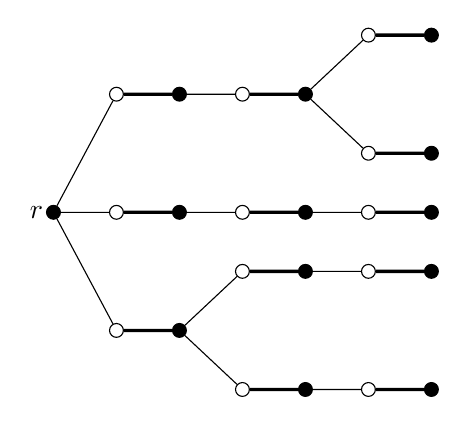
\begin{tikzpicture}
        [
            level distance=8mm,
            every node/.style={draw, fill, circle, minimum size=5pt, inner sep=0pt, line width=0.4pt},
            rootnode/.style={label=left:$r$},
            level 1/.style={nodes={fill=none}, edge from parent/.append style={line width=0.4pt}},
            level 2/.style={nodes={fill}, edge from parent/.append style={line width=1.2pt}},
            level 3/.style={nodes={fill=none}, edge from parent/.append style={line width=0.4pt}},
            level 4/.style={nodes={fill}, edge from parent/.append style={line width=1.2pt}},
            level 5/.style={nodes={fill=none}, edge from parent/.append style={line width=0.4pt}},
            level 6/.style={nodes={fill}, edge from parent/.append style={line width=1.2pt}},
            edge from parent/.style={draw}
        ]

        \node[rootnode] (root) at (0,0) {} [grow = east]
            child {node {} 
                child {node {}
                    child {node {}
                        child {node {} 
                            child {node {}
                                child {node {} 
                                }
                            }
                        }
                    }
                    child {node {}
                        child {node {} 
                            child {node {}
                                child {node {} 
                                }
                            }
                        }
                    }
                }
            } 
            child {node {} 
                child {node {}
                    child {node {} 
                        child {node {}
                            child {node {} 
                                child {node {}}
                            }
                        }
                    }
                }
            }
            child {node {} 
                child {node {}
                    child {node {} 
                        child {node {}
                            child {node {} 
                                child {node {}} 
                            }
                            child {node {} 
                                child {node {}} 
                            }
                        }    
                    }
                }
            };
    \end{tikzpicture}
    \caption{An example of an alternating tree. Nodes in $A$ are white while nodes in $B$ are black.}
    \label{fig:alternating_tree}
\end{figure}

We can divide an alternating tree $T = (V_T, E_T)$ into two node sets $A$ and $B$ such that $A$ is the set of nodes 
at the other end of an odd-length $M$-alternating path starting at $r$ and $B$ is the set of nodes at the other end 
of an even-length $M$-alternating path starting at $r$. Such sets can be built by the following relation: 
starting with $A = \emptyset$ and $B = \lrc{r}$, if $\lrp{u, v} \in E$ such that $u \in B$ and $v \notin A \cup B$ and there 
exists an edge $\lrp{v, w} \in M$, then $A \gets A \cup \lrc{v}$ and $B \gets B \cup \lrc{w}$. Note that if there exists some 
edge $\lrp{i, j}$ where $i \in B$ and $j \notin T$ such that $j$ is $M$-exposed, then the path $P = \lrp{r, v_1}, \ldots, \lrp{i, j}$
is $M$-augmenting. 

\begin{definition}
    An $M$-alternating tree is \emph{maximal} if for all $b \in B$, $\f[N]{b} \sse V_T$ (i.e.\! no additional nodes can be added to the tree).
    It is \emph{frustrated} if for all $b \in B$, $\f[N]{b} \sse A$.
    \label{def:maximal_alternating_tree}
\end{definition} 

\subsection{Maximum Matchings in the Bipartite Case}

\begin{algorithm}[!h]
    \caption{Maximum Matching in Bipartite Graphs Algorithm} \label{alg:max_match_bipartite}
    \begin{algorithmic}[1]
        \Algin A bipartite graph $G = \lrp{L, R, E}$
        \Algout A matching $M$ 
        \State $X \gets V$ \Comment{The set of $M$-exposed nodes}
    \end{algorithmic}
\end{algorithm}